\section{Estado del Arte}


{\color{orange}
La rehabilitación de los pacientes tras una lesión medular es un tema peliagudo, que conlleva un de complicaciones, ya que la rehabilitación de estos pacientes requiere de un gran esfuerzo físico y psicológico 
%\cite{Buscarla en los apuntes o en algún sitio, que seguro que está}%.
Por estos motivos, en los últimos años, un enfoque que está ganando tracción es el de las interfaces cerebro-computador (\acrshort{bci}), que permiten una rehabilitación asistida más eficiente y con una menor carga al paciente y al profesional \cite{XXX}.
}

Este capitulo trata de introducir los fundamentos que sustentan este trabajo, al igual que se ahonda en el estado actual de las técnicas de \acrfull{bci} y \acrfull{eeg} y sus aplicaciones, para de esta manera poder entender el problema que se pretende resolver y la solución que se pretende dar.


%SEPARAR ASISTENCIA DE REHABILITACIÓN% NO ES LO MISMO

\subsection{Conceptos Relevantes del Dominio}

Aqui debería poner algoooooooooooooooooooooooooooooo
Nose el qué

\subsection{Lesiones y patologías del sistema nervioso central}

El \acrfull{cns}, encargado de la planificación, iniciación y modulación del movimiento, comprende estructuras como la corteza cerebral, el tronco encefálico, el cerebelo y la médula espinal. A través de estas estructuras, el \acrshort{cns} procesa la información sensorial y genera impulsos nerviosos que son transmitidos a los músculos para producir movimiento \cite{emos_NeuroanatomyUpper2026}.

Las lesiones o patologías que afectan al \acrshort{cns} pueden dañar tanto las neuronas como las vías de comunicación entre ellas, alterando la transmisión de señales motoras y sensitivas. Como consecuencia, pueden aparecer deficiencias motoras, pérdida de sensibilidad, alteraciones del equilibrio o dificultades en la coordinación del movimiento \cite{emos_NeuroanatomyUpper2026}.

Entre las lesiones más relevantes se encuentran las \acrfull{scis}, producidas por causas traumáticas o no traumáticas que dañan parcial o totalmente la médula espinal. Este daño interrumpe la transmisión de señales nerviosas entre el cerebro y las regiones corporales situadas por debajo de la lesión. Los síntomas dependen tanto de la localización como de la gravedad del daño. Las lesiones cervicales pueden provocar tetraplegia, mientras que lesiones en regiones más bajas suelen derivar en paraplegia \cite{margetis_SpinalCord2026,ninds_SpinalCord}.

En la figura \ref{fig:spinal_cord} se puede ver un esquema de las lesiones medulares en función del area de lesión.

\begin{figure}[htbp]
    \centering
    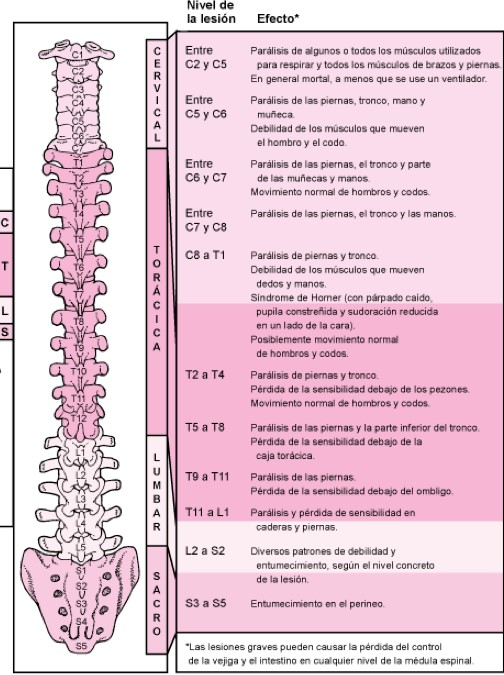
\includegraphics[width=0.80\textwidth]{img/spinal_cord_injury.png}
    %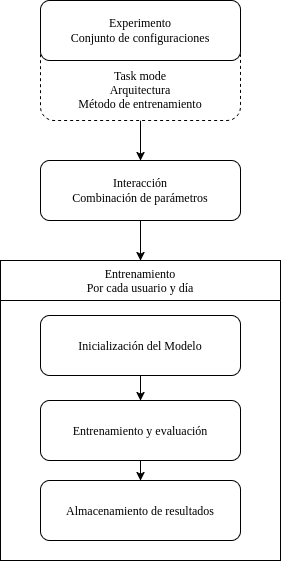
\includegraphics[height=\dimexpr\pagegoal-\pagetotal-\baselineskip\relax,width=\textwidth,keepaspectratio]{img/diagrama_pipeline.drawio.png}
    \caption{Esquema de las lesiones medulares en función del area de lesión \cite{corrallopez_TraumatismoMedular2023}}
    \label{fig:spinal_cord}
\end{figure}

Otra de las principales patologías del \acrshort{cns} son los accidentes cerebrovasculares o ictus. Estos pueden clasificarse en hemorrágicos, cuando se produce la rotura de un vaso sanguíneo cerebral, o isquémicos, cuando una obstrucción reduce o bloquea el flujo sanguíneo. En ambos casos se produce daño neuronal debido a la falta de oxígeno y nutrientes en el tejido cerebral afectado \cite{murphy_StrokeCauses2020}. Los ictus representan una de las principales causas de discapacidad motora adquirida y mortalidad a nivel mundial \cite{gao_RestoringCentral2022, emos_NeuroanatomyUpper2026, murphy_StrokeCauses2020}.

A pesar de la gravedad de estas lesiones, existe un potencial de rehabilitación en la neuroplasticidad. La neuroplasticidad la capacidad del \acrshort{cns} para modificar su estructura y funcionamiento, así como crear nuevas conexiones neuronales en respuesta a estímulos externos o internos \cite{emos_NeuroanatomyUpper2026,puderbaugh_Neuroplasticity2026}. La rehabilitación neurológica busca potenciar esta reorganización funcional de las áreas cerebrales no afectadas\cite{dipalma_FrontiersNeurorehabilitation2025}, creando nuevas conexiones mediante la repetición de tareas.

La rehabilitación constituye un proceso complejo que requiere un enfoque multidisciplinar y tratamientos personalizados. Aunque parte de la recuperación motora suele producirse durante los primeros meses tras la lesión, muchos pacientes continúan presentando secuelas permanentes en fases crónicas \cite{gao_RestoringCentral2022}. En estos casos, las tecnologías de asistencia, incluyendo los sistemas basados en interfaces cerebro-computadora (\acrshort{bci}), representan una herramienta prometedora para mejorar la autonomía y la interacción con el entorno.



\subsection{Electroencefalografía (EEG)}\label{sec:eeg}

La electroencefalografía (EEG) consiste en la captación de la actividad eléctrica cerebral generada por la comunicación entre neuronas. Estas señales se registran mediante electrodos no invasivos colocados sobre el cuero cabelludo y son posteriormente amplificadas y representadas en función del tiempo \cite{luck_IntroductionEventRelated2014,sherman_EEGSignal2020}.

Dentro de estas señales se encuentran respuestas neuronales asociadas a distintos tipos de eventos (sensoriales, cognitivos y motores) conocidas como potenciales relacionados con eventos (\acrshort{erp}), así como aquellas asociadas a la imaginación motora (\acrshort{mi}) \cite{luck_IntroductionEventRelated2014,jiang_ComprehensiveReview2026}.

Es común realizar una separación de estas señales en función de su frecuencia, ya que se ha demostrado que distintas bandas de frecuencia se corresponden con estados mentales concretos \cite{sherman_EEGSignal2020,roohi-azizi_ChangesBrains2017}.

\begin{itemize}
    \item \textbf{Delta} (\textless4 Hz): Ubicadas en la región frontal en adultos y posterior en los niños. Se asocian principalmente al sueño, siendo también frecuentes en niños y en tareas de atención sostenida.

    \item \textbf{Theta} (4--7 Hz): Predominan en las regiones parietal y temporal en niños. En adultos, aparecen durante algunas fases del sueño o en estados de estrés

    \item \textbf{Alpha} (8--13 Hz): Se localizan en la región occipital. Se asocian a estados de relajación con los ojos cerrados, disminuyendo durante la concentración y el sueño.

    \item \textbf{Beta} (13--30 Hz): Son detectadas en los lóbulos frontal y parietal y presentan una distribución relativamente simétrica. Aparecen en tareas de calma activa con los ojos abiertos. Pero también pueden aparecer durante actividad mental intensa o situaciones de estrés.

    \item \textbf{Gamma} (\textgreater30 Hz): Se han relacionado con actividad en la región somatosensorial durante tareas de procesamiento multisensorial y en procesos cognitivos complejos, como la memoria.

    \item \textbf{Mu} (8--12 Hz): Se localizan en el córtex sensoriomotor y se asocian a la actividad de este sistema en reposo.
\end{itemize}

El análisis de señales \acrshort{eeg} es una herramienta muy potente que permite revelar información sobre la actividad cerebral de un individuo, teniendo muchas aplicaciones en neurociencia y en el control de \acrshort{bci} \cite{craik_DeepLearning2019}.

Entre las principales ventajas del uso de \acrshort{eeg} se encuentran \cite{sherman_EEGSignal2020,luck_IntroductionEventRelated2014, telpaz_UsingEEG2015,schirrmeister_DeepLearning2017}:

\begin{itemize}
    \item \textbf{Alta resolución temporal}: Permite registrar cambios en la actividad cerebral en el rango de milisegundos.

          \item\textbf{Medición directa de actividad eléctrica}: A diferencia de otras técnicas que estiman la actividad cerebral de forma indirecta mediante cambios en los niveles de oxígeno en sangre, las señales \acrshort{eeg} registran directamente la actividad eléctrica generada por poblaciones neuronales.

    \item \textbf{Carácter no invasivo}: La señal puede registrarse mediante electrodos colocados sobre el cuero cabelludo, sin necesidad de procedimientos quirúrgicos. Esto reduce el riesgo de sufrir complicaciones durante la captura de la señal y las molestias a los pacientes.

    \item \textbf{Bajo coste relativo}: En comparación con otras técnicas de neuroimagen, como la resonancia magnética funcional, los sistemas \acrshort{eeg} suelen ser más accesibles y fáciles de utilizar.

\end{itemize}

Algunas de las desventajas que convierten a estas señales en difíciles de analizar son las siguientes \cite{luck_IntroductionEventRelated2014,saha_IntraIntersubject2020,klonowski_EverythingYou2009}:


\begin{itemize}
    \item \textbf{Baja resolución espacial}: Las señales \acrshort{eeg} no permiten localizar con precisión la fuente de actividad cerebral, ya que representan una media de multiples fuentes de actividad neuronales.

    \item \textbf{Variabilidad inter-sujeto e intra-sujeto}: Existe una gran variabilidad en las señales EEG entre diferentes individuos, lo que dificulta la observación de patrones en ellas. A su vez, las propiedades estadísticas de las señales pueden variar a lo largo del tiempo (son señales no estacionarias), incluso para un mismo sujeto y tarea.

    \item \textbf{Ruido}: Las señales EEG son altamente susceptibles a artefactos, como el movimiento, la actividad muscular (EMG) o interferencias externas. Además, la amplitud de las señales EEG es muy baja en comparación con el ruido presente, lo que exige un preprocesado avanzado para eliminar el ruido y mejorar la calidad de las señales.

\end{itemize}

Estas limitaciones justifican el uso de técnicas avanzadas de procesamiento y aprendizaje automático. En los últimos años el uso de modelos de aprendizaje profundo (deep learning) ha supuesto un avance significativo, facilitando el desarrollo de aplicaciones más prácticas y reduciendo la dependencia de procesamiento manual por parte de expertos \cite{craik_DeepLearning2019}.

En el contexto del aprendizaje profundo (\textit{deep learning}) surge una cuarta limitación que es la \textbf{escasez de datos} disponibles para el entrenamiento. Los algoritmos de deep learning requieren una grán cantidad de muestras para entrenar y generalizar, lo que dificulta su aplicación en tareas con pocos ejemplos.

A diferencia de otros dominios donde pueden obtenerse grandes volúmenes de datos de forma relativamente sencilla, la adquisición de señales EEG requiere equipamiento especializado, personal cualificado y una preparación cuidadosa de cada sesión experimental. Además, la anotación de los datos suele ser costosa y dependiente del protocolo utilizado \cite{tan_DeepTransfer2018}.

La recogida de datos EEG también presenta limitaciones logísticas, ya que las sesiones experimentales suelen requerir tiempos prolongados de preparación y ejecución, lo que dificulta la obtención de medidas consecutivas \cite{sugden_RemoteCollection2023}. En aplicaciones BCI, este problema se ve agravado por la fatiga física y mental de los participantes, especialmente cuando se requieren múltiples ensayos o sesiones de larga duración \cite{rommel_DataAugmentation2022}.

Como consecuencia de estas limitaciones, los conjuntos de datos EEG suelen ser significativamente más reducidos que los utilizados habitualmente en otras áreas del aprendizaje profundo.


\subsubsection{Potenciales relacionados a eventos (ERP)}

\subsubsection{Intención de movimiento (MI)}
\begin{comment}

    \begin{itemize}
    \item Qué es detectar intención
    \item Tipos de señales:
    \begin{itemize}
    \item motor imagery
    \item movimiento real 
\end{itemize}
\item Importancia en control de dispositivos
\end{itemize}

\end{comment}



\subsubsection{Interfaces Cerebro-Computador (BCI)}

Definición → 1 párrafo
Funcionamiento + figura → 2 párrafos
Aplicaciones → 1 párrafo
Tipos → 1 párrafo


Una interfaz cerebro-computador (BCI) es un sistema capaz de adquirir señales cerebrales, procesarlas y traducirlas en comandos de control para un dispositivo externo, sin necesidad de utilizar las vías motoras convencionales \cite{young_BraincomputerInterfaces2021,he_BrainComputer2020}. Inicialmente, las aplicaciones de estas interfaces se centraban en la rehabilitación y asistencia médica para la recuperación de capacidades motoras de pacientes con lesiones motoras\cite{,waldert_InvasiveVs2016,he_BrainComputer2020}.

El esquema general de las \acrshort{bci} se representa en la figura \ref{fig:esquemaBCI}. En él se observan las distintas fases de las que se compone el sistema de control. El primer paso es la adquisición de la señal cerebral, en el cual se registran los potenciales mediante electrodos posicionados en distintas zonas de la cabeza\cite{wolpaw_BraincomputerInterfaces2012}. 

Después de la adquisición de la señal, se realiza un paso intermedio en el cual se eliminan posibles artefactos de la señal, como las interferencias de red o las componentes de ruido.

A continuación estas señales son procesadas para extraer las características específicas sujeto de análisis. Es procesamiento incluye uno o varios métodos de filtrado, como el análisis espectral, la medición de la amplitud de voltajes, etc. Este 


Se trata de una tecnología capaz de ayudar en la rehabilitación de pacientes con lesiones motoras, al igual que permite reemplazar las funciones de los miembros dañados por la lesión en pacientes crónicos\cite{he_BrainComputer2020}.

The immediate goal is to provide these users, who may be completely paralyzed, or ‘locked in’, with basic communication capabilities so that they can express their wishes to caregivers or even operate word processing programs or neuroprostheses\cite{wolpaw_BrainComputer2002}.


A BCI output might replace natural output that has been lost as a result of injury or disease. For example, a person who can no longer speak might use a BCI to type words that are then spoken by a speech synthesizer. Or a person who has lost limb control might use a BCI to operate a motorized wheelchair. In these examples the BCI outputs replace lost natural outputs.  A BCI output might restore lost natural output. For example, a person with spinal cord injury whose arms and hands are paralyzed might use a BCI to stimulate the paralyzed  muscles via implanted electrodes so that the muscles move the limbs. Or a person who has lost bladder function due to multiple sclerosis might use a BCI to stimulate the peripheral nerves that control the bladder, thus enabling urination. In these examples, the BCI outputs restore the natural outputs.  A BCI output might enhance natural CNS output. For example, a person performing a task that requires continuous attention over a prolonged period (e.g., driving a vehicle or serving as a sentry) might use a BCI that detects the brain activity preceding lapses in attention and then provides an output (e.g., a sound) that alerts the person and restores attention. By preventing the attentional lapses that periodically impair natural CNS output (and might cause traffic accidents), the BCI enhances the natural output.  A BCI output might supplement natural CNS output. For example, a person who is controlling the position of a computer cursor with a hand-operated joystick might use a BCI to select items that the cursor reaches. Or a person might use a BCI to control a third (i.e., robotic) arm and hand. In these cases, the BCI supplements natural neuromuscular output with an additional, artificial output \cite{wolpaw_BraincomputerInterfaces2012}.


{
    \color{red}{
        El funcionamiento general de una BMI está representado en la Figura 4. El primer paso,  es la adquisición de los datos, donde las señales cerebrales del sujeto son registradas mediante electrodos, invasivos o no invasivos, ubicados en su cabeza y transformadas a señales digitales a través de amplificadores.  El segundo paso, es el procesamiento de las señales registradas aplicándoles una serie de filtros para eliminar ruido y otros artefactos, como las interferencias de red. Una vez acondicionada la señal, el tercer paso es extraer características de los trozos de señal y se  seleccionan aquellas que aportan información relevante para diferenciar la tarea en el clasificador.  El siguiente paso es clasificar los ritmos motores captados por los electrodos según los potenciales evocados o intenciones motoras que puedan contener. En función de la clasificación de la señal, se producen distintos comandos de control en otros dispositivos,  como pueden ser ordenadores, robots domésticos o exoesqueletos, entre otros. Tras ejecutar el comando, el dispositivo que lo ha ejecutado produce una respuesta que es transmitida al sujeto.  Generalmente, los BMI son sistemas de bucle cerrado donde el sujeto es realimentado con información acerca del resultado de las órdenes enviadas al dispositivo. La respuesta recibida varía dependiendo del dispositivo al que está vinculado la BMI. Cuando está  conectada a un ordenador recibirá un feedback visual. En cambio, cuando se trate de un exoesqueleto, la respuesta será a través de un movimiento en la extremidad del sujeto

        En primer lugar, los BMI invasivos consisten en introducir los electrodos en la región intracortical de la cabeza. Este procedimiento implica una operación donde se retira un trozo de cráneo para implantar los electrodos en el cerebro y pinchar las neuronas. La  principal ventaja de esta técnica es que la adquisición de la señal se hace directamente sobre las neuronas que producen las señales deseadas. Por tanto, la señal tiene una gran resolución espacial y temporal con escaso ruido. Sin embargo, esta técnica presenta una importante desventaja que es exponer al paciente a una intervención quirúrgica compleja  y a electrodos en el interior de su cuerpo, que tarde o temprano deben ser o bien reemplazados, o bien retirados.  En segundo lugar, los BMI parcialmente invasivos colocan los electrodos sobre la superficie del cerebro. Esta técnica es muy similar a la anterior, pero en este caso la captación se realiza por electrocorticografía (ECoG) [15]. Este método presenta una resolución espacial y temporal medias, ya que eliminan parte de los artefactos causados  por la piel y el hueso, pero las señales de las regiones más profundas del cerebro siguen presentando una pequeña cantidad de ruido espacial. Por el contrario, la principal  Figura 9. Posición de los electrodos en la cabeza para la adquisición de las señales EEG. [4] 13 desventaja que presentan es exactamente la misma que en las BMI invasivas: la  intervención quirúrgica y sus riesgos. Adicionalmente, ambas técnicas implican un elevado coste.  En tercer lugar, los BMI no invasivos ubican los electrodos en la superficie de la cabeza, sobre el cuero cabelludo. Por tanto, se elimina el problema de someter al paciente a la cirugía y se reduce el coste. Además, los electrodos son portables, normalmente están  agrupados en un casco, y se puede colocar en distintos entornos, no sólo en un quirófano. Sin embrago, el tiempo de colocación de los electrodos es muy elevado. Asimismo, la desventaja de eliminar los electrodos no invasivos es que se pierde resolución espacial, especialmente al realizar la captación por EEG o MEG, donde algunos electrodos registran señales de múltiples regiones. No obstante, este método no pierde la resolución temporal
    }
}


\begin{figure}[htbp]
    \centering
    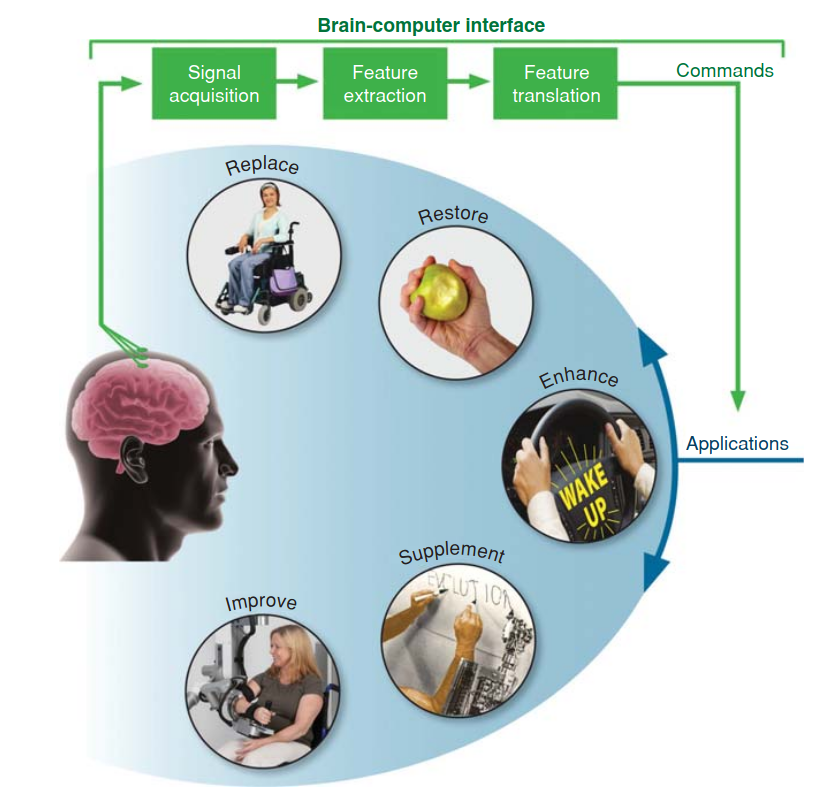
\includegraphics[width=0.90\textwidth]{img/bci_schema.png}
    %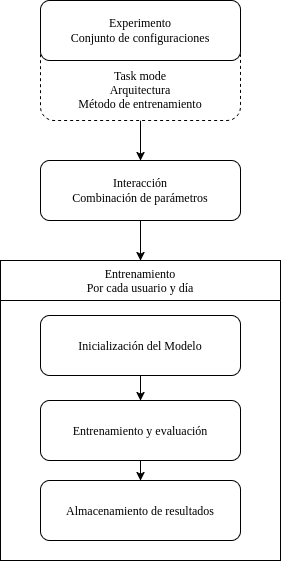
\includegraphics[height=\dimexpr\pagegoal-\pagetotal-\baselineskip\relax,width=\textwidth,keepaspectratio]{img/diagrama_pipeline.drawio.png}
    \caption{Esquema general del funcionamiento de una BCI \cite{wolpaw_BraincomputerInterfaces2012}}
    \label{fig:esquemaBCI}
\end{figure}


SACAR COSAS DE \cite{lawhern_EEGNetCompact2018}

{\color{red}
Como tecnología asistiva
Cuando el daño motor de un individuo ya es crónico, estas
interfaces se pueden utilizar como herramienta de comunicación,
para controlar miembros artificiales (sustitución motora) o incluso
para el ocio

Sustitución motora

• El concepto de movilidad asistiva se puede encuadrar dentro de la
sustitución motora
• Un ejemplo es el uso de sillas de ruedas controladas por BCI
• La silla de ruedas, es considerada, por muchos usuarios como
parte de su propio cuerpo (embodiment) y funciona de forma
equivalente a una prótesis}

\begin{figure}[H]
    \centering
    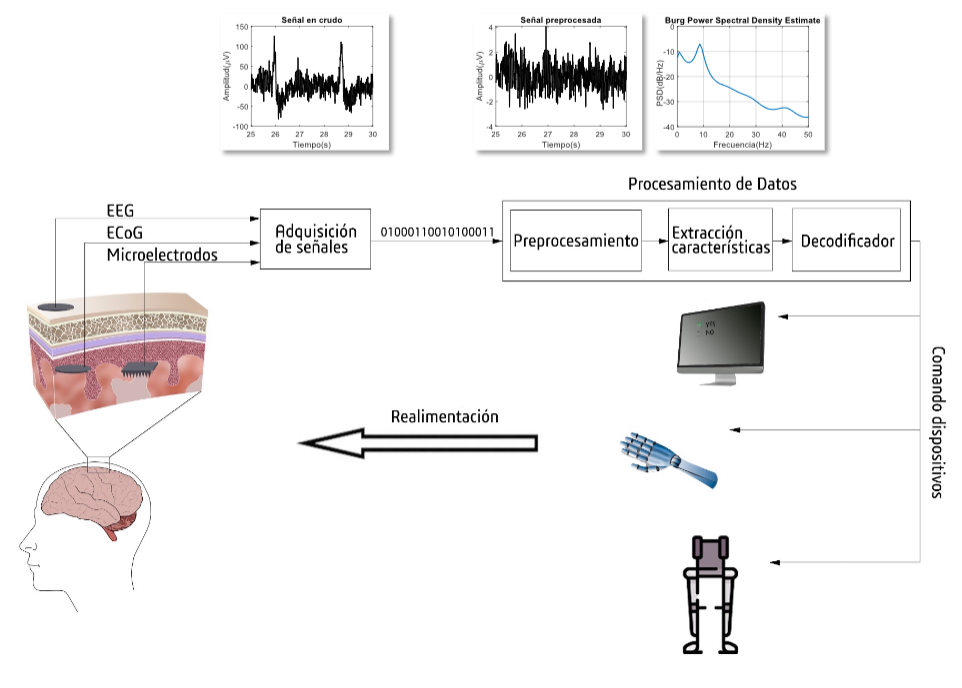
\includegraphics[width=0.90\textwidth]{img/esquema_bci.png}
    %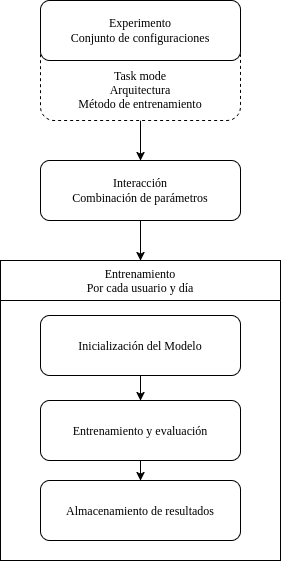
\includegraphics[height=\dimexpr\pagegoal-\pagetotal-\baselineskip\relax,width=\textwidth,keepaspectratio]{img/diagrama_pipeline.drawio.png}
    \caption{Esquema general de una BCI \cite{azorinpoveda_Tema322024}}
    \label{fig:pbci_esquema}
\end{figure}

\begin{comment}

    \begin{itemize}
    \item Qué es
    \item Pipeline típico:
    \begin{itemize}
    \item adquisición → preprocesado → clasificación → acción
\end{itemize}
\end{itemize}
\end{comment}








\subsection{Redes neuronales convolucionales}

Las redes neuronales convolucionales (\acrshort{cnn}) constituyen una de las arquitecturas de aprendizaje profundo más empleadas para el análisis de datos complejos. Aunque fueron desarrolladas originalmente para tareas de visión artificial, su capacidad para extraer características relevantes de manera automática y eficiente las ha convertido en una herramienta ampliamente utilizada en ámbitos como: el procesamiento de imágenes, el reconocimiento de voz, el procesamiento del lenguaje natural y, más recientemente, el análisis de señales biomédicas como el electroencefalograma (\acrshort{eeg}) \cite{albawi_UnderstandingConvolutional2017,lecun_DeepLearning2015,edelman_NonInvasiveBrainComputer2025,schmidhuber_DeepLearning2015}.

La operación en la que se basan estas redes es la convolución, una transformación matemática que aplica pequeños filtros o \textit{kernels} sobre la entrada para detectar patrones específicos. Cada filtro aprende durante el entrenamiento a responder a determinadas características presentes en los datos, generando como salida un conjunto de mapas de características (\textit{feature maps}). Estos \textit{feature maps} se vuelven progresivamente más abstractos y complejos conforme se avanza en la red, lo que le permite aprender automáticamente las características más discriminativas para la tarea de clasificación. Las capas convolucionales requieren un número significativamente menor de parámetros que las capas completamente conectadas (\textit{fully connected}), reduciendo el coste computacional y favoreciendo la capacidad de generalización del modelo \cite{albawi_UnderstandingConvolutional2017,edelman_NonInvasiveBrainComputer2025,lecun_DeepLearning2015,goodfellow_DeepLearning2016}.

Habitualmente, una CNN está formada por una sucesión de capas convolucionales y capas de reducción dimensional (\textit{pooling}), seguidas de una o varias capas \textit{fully connected}. Las capas convolucionales se encargan de extraer características relevantes de la señal de entrada, mientras que las capas de \textit{pooling} reducen la dimensionalidad de las representaciones obtenidas y contribuyen a disminuir el sobreajuste. Finalmente, las capas \textit{fully connected} utilizan las características extraídas para realizar la clasificación o regresión correspondiente \cite{albawi_UnderstandingConvolutional2017,rakhmatulin_ExploringConvolutional2024}.

En el ámbito de las interfaces cerebro-computador (\acrshort{bci}), las CNN se han consolidado como una de las técnicas más utilizadas para la decodificación de señales EEG \cite{craik_DeepLearning2019,schirrmeister_DeepLearning2017,edelman_NonInvasiveBrainComputer2025}. A diferencia de las imágenes, las señales EEG presentan simultáneamente una dimensión temporal y una dimensión espacial asociada a la distribución de los electrodos sobre el cuero cabelludo. Por este motivo, las arquitecturas diseñadas para EEG suelen combinar convoluciones temporales, encargadas de extraer información espectral y patrones dependientes del tiempo, con convoluciones espaciales que modelan las relaciones entre los distintos canales de la señal \cite{edelman_NonInvasiveBrainComputer2025}.

Tradicionalmente, los sistemas BCI basados en EEG dependían de técnicas de extracción manual de características combinadas con clasificadores convencionales. Sin embargo, la aparición de arquitecturas de redes neuronales profundas específicas para EEG, como DeepConvNet y ShallowConvNet, supuso un cambio de paradigma al integrar de forma conjunta las etapas de extracción de características y clasificación dentro de una misma red neuronal \cite{schirrmeister_DeepLearning2017,kollod_DeepComparisons2023}.


\subsection{Relación con Proyectos Similares}

Estructura muy clara:
\subsubsection{Métodos clásicos}

{\color{orange}
Esto investigarlo más y ponerlo bonito
Barachant et al. [22] introduced Riemannian geometry for BCI with an LDA classifier to successfully classify EEG covariance matrices. Lotte and Guan [23] introduced a unifying theoretical framework for regularizing the CSP and compared it with 10 other regularized versions of the CSP algorithm. Another feature extraction algorithm, considering the CSP, is the Filter Bank Common Spatial Pattern  (FBCSP) with a Naïve Bayesian Parzen Window classifier  \cite{kollod_DeepComparisons2023}

The winner of the BCI discipline of the Cybathlon competitions used the power spectral density of the EEG signals as a feature [13], [19] with a Gaussian classifier.
}

\begin{itemize}
    \item LDA, SVM
    \item Features manuales
    \item Limitaciones
\end{itemize}

\subsubsection{Deep Learning aplicado a EEG}

Kollod et al. \cite{kollod_DeepComparisons2023} realizaron una comparación exhaustiva de diferentes arquitecturas de aprendizaje profundo aplicadas a señales EEG, incluyendo modelos ampliamente utilizados como EEGNet, DeepConvNet y ShallowConvNet. Además de comparar el rendimiento de las distintas arquitecturas, los autores analizaron diferentes estrategias de entrenamiento, incluyendo enfoques within-subject y técnicas de transferencia de aprendizaje basadas en preentrenamiento inter-sujeto y posterior ajuste fino sobre el sujeto objetivo. Este trabajo resulta especialmente relevante para el presente estudio, ya que evalúa tanto las arquitecturas utilizadas como estrategias de entrenamiento similares a las implementadas en esta investigación.



kollodDeepComparisons2023 $\rightarrow$ hace una comparación entre varios modelos y tipos de entrenamiento 

{\color{orange}
Before neural networks, scientists intended to investigate and develop hand-crafted feature extraction methods combined with simple classification algorithms. \cite{kollod_DeepComparisons2023}
With the introduction of the Deep and Shallow ConvNets, a new trend started in BCI development. The focus had been shifted from hand-crafted features to creating neural networks which not just classify the signal but also include the feature extraction step. \cite{lawhern_EEGNetCompact2018} introduced the EEGNet, which was inspired by former neural networks that were designed for EEG signal processing, including MI-based BCIs \cite{schirrmeister_DeepLearning2017}, \cite{sakhavi_LearningTemporal2018,tabar_NovelDeep2016}. $\rightarrow$ Uso las redes de schirrmeister en el estudio.

It was demonstrated that EEGNet makes a similar feature extraction as the FBCSP This neural network inspired many scientists, which resulted in many improved versions of the EEGNet [29]–[42], \cite{kollod_DeepComparisons2023} $\rightarrow$  Esto es importante, ya que utilizo la eegNet

Other publications outside the EEGNet family [43]–[49] highlight the importance of neural network-based BCI research.

26-28  29-42 42-49


Along with the development of neural networks, scientists started investigating the effect of transfer learning [50]. This method aims to transfer knowledge between two domains and increase the classification’s accuracy. Khademi et al. [51]

This way, they aimed to transfer the knowledge of image classification and use it on spatial EEG images generated with continuous wavelet transformation method using complex Morlet mother wavelet

nother strategy is to utilize the entire EEG dataset and combine cross-subject and within-subject training, as presented in [49], [52], [53]  $\rightarrow$  Esto es importante, ya que los entrenamientos elegidos para el estudio son similares.

In this case, the knowledge is granted from subjects not used in the test set of the neural network. The network is pretrained on data from all but one subject, as it would in a cross-subject training procedure. But then the data of the test subject is also split to train and test set, as in the within-subject, and the training part is used for fine-tuning the pretrained neural network. We selected the later version of transfer learning because it is architecture independent and aimed to use it after artifact filtering.


Next to the subject-wise learning, we also investigated the effect of transfer learning. First, test subjects were selected as distinct groups of 10. The remaining subjects, called pre-train subjects, were used to set the initial optimal weights for the neural networks. A validation set was separated from the pre-train data to use it with our modified early stopping and model-saving strategy. When the pretraining phase converged, either reaching the maximum training epoch number or stopping it by the early stopping strategy, the best weights of the network were stored. For each test subject, 5-fold withinsubject cross-validation $\rightarrow$  esto es bastante parecido a uno de los métodos de entrenamiento que uso

}
    CNNs (EEGNet, DeepConvNet…)

    Qué han conseguido

    Problemas abiertos:

        generalización

        dependencia del usuario

\subsubsection{Aplicaciones en exoesqueletos / rehabilitación}

    Uso de BCI para control

    Problema clave:

        detección fiable de intención

\subsubsection{Limitaciones actuales}

    variabilidad entre sujetos

    necesidad de recalibración

    falsos positivos peligrosos

    falta de evaluación en escenarios realistas

\subsubsection{Propuesta}

En este contexto, este trabajo se centra en…

Aquí conectas directamente con tu TFM:

    comparación de métodos de entrenamiento

    evaluación pseudo-online

    análisis sistemático
